\subsection{Konfiguracja rzeczywista}
\label{subsec:konfiguracja-urzadzen}

\begin{figure}
    \centering
    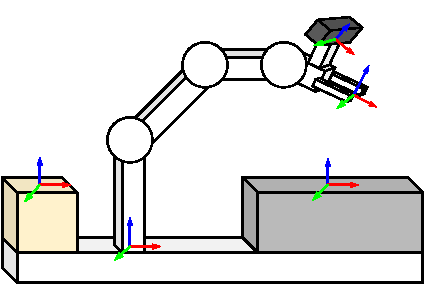
\includegraphics[width=\columnwidth]{figures/ISR-system-overview.pdf}
    \caption{Środowisko robocze projektowanego systemu}
    \label{fig:srodowisko-robocze}
\end{figure}

Projektowany system składa się z:\begin{itemize}
    \item sześciostopniowego manipulatora,
    \item chwytaka dwustanowego,
    \item kamery RGB-D,
    \item ruchomego taśmociągu,
    \item palety do odstawiania sześcianów.
\end{itemize}

Pozycja tych komponentów została przedstawiona na rysunku~\ref{fig:srodowisko-robocze}. Wszystkie transformacje pomiędzy poszczególnymi układami współrzędnych komponentów są znane.

\subsection{Agentowa struktura systemu}
\label{subsec:agentowa-struktura}

W~systemie można wyróżnić dwóch agentów: agenta $a_{1}$ wykonującego zadanie i~sterującego ramieniem, chwytakiem i~kamerą oraz agenta $a_{2}$.  Diagram komunikacji pomiędzy agentami został przedstawiony na rysunku~\ref{fig:agenty-system}. Zgodnie z~poleceniem, definicja agenta $a_{2}$ zostanie pominięta.

\begin{figure}[b]
    \centering
    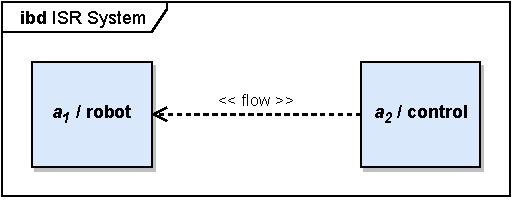
\includegraphics[width=\columnwidth]{figures/ISR-agents.pdf}
    \caption{Dekompozycja systemu na agenty}
    \label{fig:agenty-system}
\end{figure}

\begin{figure}[t]
    \leftskip-0.5em
    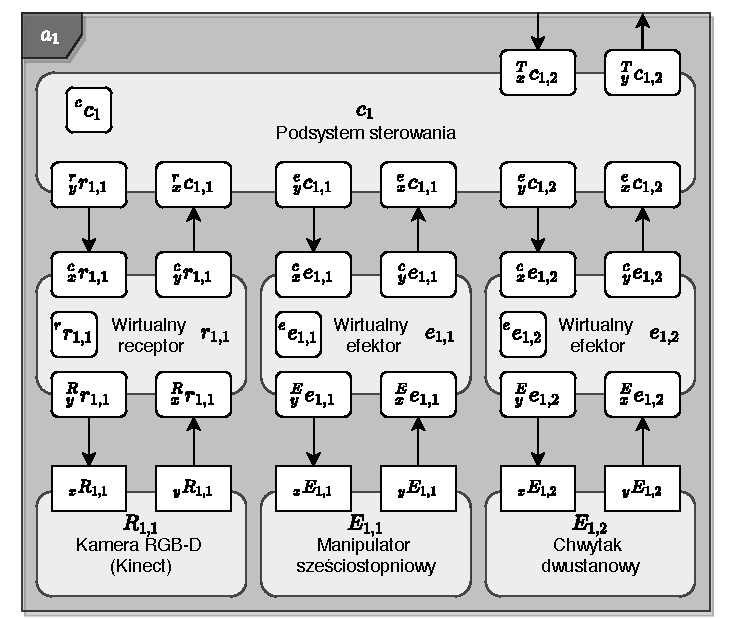
\includegraphics[width=1.05\columnwidth]{figures/ISR-agent-decomposition.pdf}
    \caption{Dekompozycja agenta $a_{1}$ na wirtualne i~rzeczywiste receptory i~efektory}
    \label{fig:dekompozycja-agent-1}
\end{figure}

Agent $a_{1}$ steruje dwoma efektorami: sześciostopniowym manipulatorem oraz dwustanowym chwytakiem, a~także odbiera dane z~jednego receptora: kamery RGB-D. Agenta $a_{1}$ zdekomponowano zgodnie z~formalizmem przedstawionym na wykładzie, na podsystem sterowania, wirtualne receptory i~efektory oraz rzeczywiste receptory i~efektory. Na rysunku~\ref{fig:dekompozycja-agent-1}, przedstawiono podział na poszczególne podsystemy, wraz z~odpowiadającymi buforami komunikacyjnymi.